\documentclass[a4paper,12pt]{report}
\usepackage[spanish, es-tabla]{babel}
\usepackage[utf8]{inputenc} 
\usepackage[margin=1in]{geometry}%margenes
\usepackage{graphicx}
\usepackage{setspace}
\onehalfspace %para espacio y medio
\setlength\parindent{0pt}%elimina sangria
\pagenumbering{gobble}%elimina nro de pag
\usepackage{natbib}%para reducir espacio entre items de la biblo


\begin{document}

{\large \textbf{Título:}} “Análisis de Identificadores para Abstraer conceptos del Dominio del Problema”
\vskip0.5cm
{\large \textbf{Autor:}} Javier Azcurra Marilungo.
\vskip0.5cm
{\large \textbf{Dirección:}}
\begin{itemize}
\itemsep0em%reduce espacio
\item \textbf{Director:} Dr. Mario Marcelo Berón.

\item \textbf{Co-Director:} Dr. Germán Antonio Montejano.
\end{itemize}

{\large \textbf{Objetivos:}} Los objetivos principales de este trabajo final de Licenciatura son:



\begin{itemize}
\itemsep0em%reduce espacio

\item Extraer identificadores de programas escritos en lenguaje JAVA.

\item Extraer comentarios y literales de programas escritos en lenguaje JAVA.

\item Analizar los identificadores capturados con ayuda de la información extraída en el ítem anterior.

\item Construir en JAVA una herramienta que implemente los ítems anteriores.

\item Evidenciar una aproximación que relacione la salida de un programa con los elementos involucrados que producen dicha salida.

\end{itemize}
{\large \textbf{Antecedentes:}}
\vskip0.5cm
%\hspace{0.5cm}  %Sangria
\hspace{0.5cm} La Comprensión de Programas (CP) \cite{BRM10,MPMR07,MBPHRU10,MAS05} es un área de la Ingeniería de Software cuyo objetivo 
principal es desa\-rrollar métodos, técnicas y herramientas que faciliten al programador 
el entendimiento de las funcionalidades de los sistemas de software.
Una forma de alcanzar este objetivo consiste en relacionar el Domino del Problema, 
es decir la salida del sistema, con el dominio del programa, o sea 
con las partes del programa utilizadas para generar la salida del sistema \cite{VMAVA95,MPOB03,BROOK82,AMPM11}.
La construcción de esta relación representa el principal desafío en el contexto de la 
CP. 

\hspace{0.5cm}Una posible solución al desafío previamente mencionado, consiste en construir 
una representación para cada dominio, luego se procede a vincular ambas representaciones a través de una estrategia de vinculación.
Para construir la representación del dominio del problema y la del dominio del programa, se necesita extraer información 
estática y dinámica propia de ambos dominios. En la actualidad se conocen distintas técnicas y herramientas que llevan a cabo esta tarea \cite{AHUL06,THBE99}.
 
\hspace{0.5cm}La información dinámica se extrae del sistema en tiempo de ejecución \cite{THBE99, TERD01}. Las técnicas encargadas de extraer este tipo de información, insertan sentencias nuevas en el código fuente del programa. Esta inserción no altera la funcionalidad original del programa. La finalidad de las nuevas sentencias es registrar las actividades realizadas durante la ejecución del programa. 

\hspace{0.5cm}Las sentencias nuevas insertadas pueden simplemente imprimir las secciones que se están ejecutando. Más complejo aún, se pueden agregar un conjunto de sentencias nuevas que reemplacen a otro conjunto (sin alterar la funcionalidad original) para hacer un estudio más preciso en ciertas partes del código.

\hspace{0.5cm}El volumen de información extraída puede ser de gran magnitud. Es por esto, que el encargado de hacer el análisis dinámico debe conocer con claridad los lugares estratégicos donde colocar las sentencias.

\hspace{0.5cm}La instrumentación de código es una de las técnicas más conocidas del análisis dinámico \cite{THBE99}. Esta técnica, inserta sentencias para crear trazas de ejecución en distintas partes del código. Las trazas clarifican la ejecución del programa mejorando la comprensión del mismo.

\hspace{0.5cm}El análisis estático es tan importante como el análisis dinámico. El análisis estático a diferencia del dinámico, no requiere ejecutar el sistema. Para realizar el análisis estático, se extrae información presente en el código utilizando técnicas de compilación tradicionales, estas técnicas realizan un análisis sintáctico y semántico en el código fuente \cite{TERD01, AHUL06}.

\hspace{0.5cm}Para llevar a cabo estos análisis se recorre el árbol de sintaxis abstracta (ASA) \cite{AHUL06}. En la fase de compilación, el ASA se construye a medida que se analiza el código.

\hspace{0.5cm}Una forma de construir el ASA es por comprensión \cite{AHUL06}, esta forma se logra en la etapa del análisis sintáctico durante el proceso de compilación del código. Es la más sencilla y se utiliza en tareas de chequeos de tipos, generación de código, construcción de grafo de funciones, entre otras.

\hspace{0.5cm}Otra forma de elaborar el ASA es por extensión \cite{AHUL06}, esta forma se usa para hacer análisis más complejos en el código. También extrae mayor cantidad de información en tiempo de compilación. Algunos ejemplos de tareas que se pueden realizar son, extracción de identificadores, extracción de funciones y tipos y demás objetos presentes en el código. 

\hspace{0.5cm}El ASA por extensión también se usa para resolver conflictos a nivel semántico, como es el caso de borrar referencias a variables redundantes, detectar funciones o estructuras a través del uso de punteros.

\hspace{0.5cm}El correspondiente trabajo hará más énfasis en la extracción de información estática. Cabe destacar que la dinámica también es importante, sin embargo su análisis requiere de otro tipo de aproximaciones que escapan a los objetivos de este trabajo. 

\hspace{0.5cm}Como bien se explico en párrafos precedentes, se pueden extraer distintos objetos del código fuente de forma estática usando técnicas de compilación, y sin la necesidad de ejecutar el código. 

%=======================================

\hspace{0.5cm}Un elemento estático que abunda en los códigos son los identificadores. Estudios realizados sobre 2.7 millones de lineas de código escritas en JAVA, indican que más del 70\% de los caracteres del código fuente forman parte de un identificador \cite{DFPM05,DMDJ13}.

\hspace{0.5cm}Los identificadores normalmente están conformados con abreviaturas en su nombramiento. Estudios realizados \cite{BCPT99,LFBEX07,EZH08,EHPV09} arrojan que detrás de las abreviaturas se encuentra oculta información importante del dominio del problema.

\hspace{0.5cm}Por lo antedicho, construir herramientas que puedan extraer y analizar identificadores desde los códigos JAVA es un gran aporte al área de CP. Una forma de analizar identificadores consiste en desplegar la información oculta de sus abreviaturas. Para lograr este cometido, primero se necesita dividir las distintas abreviaturas que el identificador compone. Por ejemplo: \textsf{inp\_fl\_sys} $\rightarrow$ \textsf{inp fl sys}. Luego se someten a un proceso de expansión. Por ejemplo: \textsf{inp fl sys} $\rightarrow$ \textsf{input file system}.

\hspace{0.5cm}Para realizar los pasos de división y expansión se recurren a fuentes de palabras/frases dentro del código: comentarios, literales strings, documentación \cite{JDPH08}. En caso de que estas fuentes escaseen, una alternativa viable es consultar fuentes de palabras externas al código como es el caso de los diccionarios con palabras en lenguaje natural, entre otros.

\hspace{0.5cm}En la actualidad existen técnicas/herramientas que extraen, dividen y expanden identificadores \cite{EZH08, EHPV09, BCPT00, HDD06}. Sin embargo, no abundan herramientas que integren todas estas tareas. A su vez, tampoco existen muchas herramientas que permita utilizar distintas políticas de división y expansión de abreviaturas, de esta forma, se podría variar los resultados obtenidos y determinar el más adecuado.

\hspace{0.5cm}En base a lo descripto en los párrafos anteriores, en el presente trabajo final de licenciatura se elaborará un analizador sintáctico en lenguaje JAVA que extrae los identificadores, comentarios y literales encontrados en códigos fuentes escritos en lenguaje JAVA.

\hspace{0.5cm}Luego se va investigar técnicas conocidas de división y de expansión de abreviaturas pertenecientes a identificadores. Finalmente, se procederá a implementar una herramienta que integre las técnicas de análisis de identificadores antedichas junto al analizador sintáctico explicado en el párrafo anterior. De esta manera, se obtendrá una herramienta que extrae y analiza información estática contenida detrás de los identificadores. Extraer y analizar este tipo de información propia del dominio del problema \cite{DFPM05,DMDJ13,EHPV09} es un aporte importante para encarar uno de los desafíos principales de la CP: vincular el Dominio del Problema con el Dominio del Programa.
\vskip0.5cm


{\large \textbf{Metodología:}}
\vskip0.5cm

\hspace{0.5cm}La metodología a utilizar en este trabajo final, esta enmarcada por 3 etapas principales:

\begin{itemize}
\renewcommand{\labelitemi}{$\circ$}%icono circulo
\itemsep0em%reduce espacio
\item \textbf{Primera Etapa: Investigación de conceptos orientados a la Comprensión de Programas y a la extracción de información estática.}

\hspace{0.5cm}En esta etapa se incorporan los conocimientos necesarios para llevar adelante este trabajo final. Se investigará sobre comprensión de programas y las áreas que contiene. De todas estas áreas, se hará más hincapié en la extracción de información estática en base al análisis de identificadores presentes en los códigos. Este análisis, servirá para la elaboración de técnicas de comprensión de sistemas.

\pagebreak
\item \textbf{Segunda Etapa: Elaboración del analizador sintáctico que extrae\\identificadores de los códigos escritos en JAVA.}

\hspace{0.5cm}Se construirá un analizador sintáctico (parser) encargado de extraer identificadores, comentarios y literales desde los códigos escritos en JAVA. Estos comentarios y literales ayudarán al análisis de identificadores. Para construir este parser, se investigarán herramientas que ayude a la construcción y se elegirá la más adecuada. Se llevarán a cabo las pruebas pertinentes.

\vskip0.5cm
\item \textbf{Tercera Etapa: Construcción de la herramienta que analiza\\identificadores e integra el parser elaborado en la etapa previa.}

\hspace{0.5cm}Finalmente, en la última etapa se construye una herramienta que contendrá al analizador sintáctico elaborado en la etapa anterior y también implementa algunas de las técnicas de análisis de identificadores estudiadas en la primer etapa. La finalidad de esta herramienta es extraer y analizar información presente en identificadores ubicados en códigos JAVA. Esta información extraída y analizada, se considera propia del Dominio del Problema y es un aporte a la reconstrucción de la relación entre: el Dominio del Problema y el Dominio del Programa.

\end{itemize}

{\large \textbf{Plan y cronograma de tareas:}}

\begin{enumerate}
\itemsep0em%reduce espacio
\item Estudiar conceptos, técnicas y herramientas sobre la comprensión de programas: con esto se lográ conocer las características relacionadas al ámbito de la comprensión de sistemas.

\item\label{plan1} Investigar conceptos, técnicas y herramientas relacionados al análisis de identificadores: aquí se adquieren los conceptos necesarios para extraer información del Dominio del Problema, en base a los identificadores.

%\item Estudiar herramientas automatizadas que generen Analizadores Lexicográficos y Analizadores Sintácticos, se hará preferencia en aquellas que usen gramática de atributos.

\item Investigar herramientas que ayuden a construir un Analizador Sintáctico (parser). Preferentemente se escogerán aquellas que empleen gramáticas de atributos \cite{AHUL06}.

\item Estudiar la gramática de JAVA e implementar el Analizador Sintáctico (parser) utilizando alguna herramienta investigada del item anterior.

\item Implementar una herramienta en JAVA que  contenga distintas técnicas de análisis de identificadores investigados en el ítem \ref{plan1}. Esta herramienta también contendrá el parser elaborado en la etapa anterior.

\item Escribir el informe del trabajo final. Mientras se ejecutan los ítems precedentes, se irá redactando el informe correspondiente al trabajo final.
\end{enumerate}


\begin{figure}[t] %[h] para here [b] para bottom [t] para top
\centerline{%queda centrada mejor la imagen
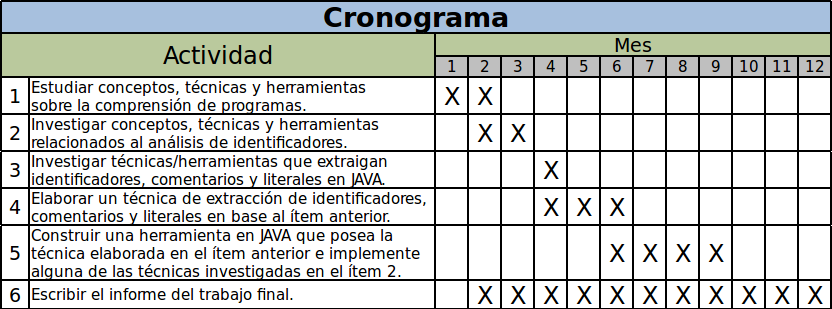
\includegraphics[scale= 0.85]{./crono.png}
}
\end{figure} 

\pagebreak
{\large \textbf{Recursos:}}
\vskip0.5cm
\hspace{0.5cm}El correspondiente trabajo final se llevará a cabo en la Universidad Nacional de San Luis, en el Área Programación y Metodologías de Desarrollo de Software enmarcado en los siguientes proyectos:

\begin{itemize}
\renewcommand{\labelitemi}{$\diamondsuit$}%icono circulo
\itemsep0em%reduce espacio
\item \textit{“Ingeniería del Software: Conceptos Métodos Técnicas y 
Herramientas en un Contexto de Ingeniería de Software en Evolución”} de la Universidad 
Nacional de San Luis. 
Dicho proyecto, es reconocido por el programa de incentivos y es la continuación de 
diferentes proyectos de investigación de gran éxito a nivel nacional e internacional.

\item “Quixote - Development of Problem Domain Models to Interconnect the Behavioral and Operational Views to Aid in Software Systems Comprehension” (código de proyecto: PO/09/38).  Quixote es un proyecto bilateral entre la Universidade do Minho (Portugal) y la Universidad Nacional de San Luis (Argentina). Dicho proyecto fue aprobado por el Ministerio de Ciencia, Tecnología e Innovación Productiva de la Nación (MinCyT)\footnote[1]{www.mincyt.gov.ar/}, y la Fundação para a Ciência e Tecnología (FCT)\footnote[2]{www.fct.mctes.pt/} de Portugal. 

\end{itemize}

\hspace{0.5cm}Ambos entes soportan económicamente la realización de diferentes misiones de investigación desde Argentina a Portugal y viceversa, como así también la presentación y publicación de artículos en diferentes congresos nacionales e internacionales.\\

\hspace{0.5cm}Por otro lado, el equipamiento necesario es una PC con el sistema Linux, impresora y papel para realizar las impresiones del informe. También se hará uso de internet, de material bibliográfico provisto por la biblioteca “Antonio Esteban Agüero”; y  de material provisto por las librerías digitales a las que se tiene acceso desde la Universidad.



%========================================

\renewcommand{\bibname}{\vspace{-2.5cm} \large \textbf{Bibliografía}}
\setlength{\bibsep}{1.5pt}
\bibliographystyle{plain}%{alpha}
\bibliography{biblo}
\nocite{*}%para que imprima toda la referencias sin necesidad de citar

{\large \textbf{\\\\Firma de alumno y asesores}}

\end{document}